\chapter{LoRa}
\section{LoRa}
Tra tutte le tecnologie che cercano di predominare il network layer, LoRaWAN, è
quella che si presta di più alla sperimentazione.
Grazie al protocollo di natura open e la facile reperibilità dei moduli radio e  
sono necessari solo un gateway e dei sensori per creare le prime applicazioni.

\section{Narrow Band e Spread Spectrum}
Il successo delle tecnologie LPWAN risiede nella loro abilità di offrire una
connessione a bassa potenza per un grande numero di devices distribuiti in una
vasta area geografica. Per capire il principio di funzionamento alla base del
layer fisico LoRa, e necessario comprendere il tipo di modulazione utilizzata e
i vantaggi che ne derivano.
Le principali tecniche di modulazione utilizzate dalle reti LPWA sono in grado
di offrire un bilanci di collegamento (link budget ) pari a 150$\pm$ 10[dB], il quale
garantisce un range di operatività pari ad una decina di chilometri.
Andando a ridurre il data rate è possibile concentrare più energia in ogni
simbolo trasmesso. In questo modo il gateway è in grado di decodificare segnali
molto attenuati. In generale le tecnologie LPWAN sono in grado di decodificare
segnali attenuati fino a -130[dBm]. Per ottenere questi risultati due tipi di
modulazione sono stati utilizzati da LPWAN diverse.

\subsection{Narrow Band}
La modulazione narrowband codifica il segnale in una banda molto ristretta (
 $\approx$25[KHz] ), in questo modo è in grado di ottenere alte prestazioni nel
bilancio di collegamento. Assegnando ad ogni frequenza una banda molto
ristretta, la NB è in grado di utilizzare l'intero spettro in maniera efficace.
Il livello di rumore all'interno di ogni canale \improvement{Trovare un termine più
adatto } è molto basso, rendendo semplice la demodulazione da parte del gateway.
Per aumentare la capacità del singolo nodo e diminuire la complessità dei moduli
radio SigFox e altre tecnologie  estremizzano il concetto di narrowband andando a assegnare ad
ogni portante una banda di appena 100[Hz]. Inequivocabilmente il data rate
diminuisce di molto e il tempo il quale il ricevitore deve rimanere acceso
aumenta. 

\subsection{Spread spectrum} 
Come dice il nome, la tecnica spread spectrum è in grado di distribuire un
segnale narrowband in un campo di frequenze più vasto del necessario, mantenendo
però la stessa densità di potenza.
Come risultato otteniamo una trasmissione che incorpora più rumore di una
trasmissione NB, riuscendo però ad essere molto più resistente alle interferenze
ed agli attacchi basati sul jamming.
Per la natura rumorosa del segnale, il ricevitore dovrà compiere uno sforzo
maggiore per la ricezione del segnale, il quale molto spesso sarà ricevuto sotto
il noise floor \improvement{Noise floor in italiano?}
Per ottimizzare l'uso dello spettro, è possibile inviare segnali codificati con
frequenze ortogonali , in questo modo è possibili decodificare in maniera
concorrente segnali diversi, andando ad aumentare la capacità della rete.

\begin{figure}[h]
\centering 
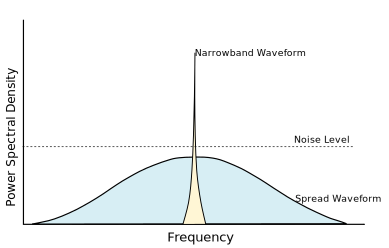
\includegraphics[width=11cm]{spread_spectrum_temp}
\caption{Comparazione tra UNB e SSP}
\end{figure}

\section{CSS}
CSS o Chirp Spread Spectrum è la modulazione alla base del layer fisico LoRa. 
Con Chirp (Compressed High Intensity Radar Pulse) si intende un segnale di
ampiezza costante, il quale incrementa o decrementa la sua frequenza nel tempo.
Parliamo quindi di \emph{UpChirp} nel caso di un aumento di frequenza e di
\emph{DownChirp} nel caso di un decremento.
I l'utilizzo di segnali di tipo Chirp non è nuovo nel campo delle
telecomunicazioni; infatti, questa tecnica di compressione del segnale, 
è molto utilizzata in applicazioni radar o  sonar  poiché tramite essa è possibile aumentare il range
di risoluzione spaziale e il rapporto segnale rumore.
Il più generico segnale chirp può essere rappresentato da una sinusoide che come
argomento ha una funzione $\theta(t)$ che varia in funzione del tempo.
\begin{equation}\label{eq:1}
        s(t) = A\cos(\theta (t))
\end{equation}
Derivando ora l'argomento di $s(t)$ nel tempo, possiamo andare a definire due
nuovi paramentri, la frequenza istantanea $\gamma(t)$ \ref{eq:2} ed un parametro che
chiameremo chirpizzazione istantanea $c(t)$ \ref{eq:3}.
\begin{equation}\label{eq:2}
        \gamma(t) = \frac{1}{2\pi} \frac{d\theta(t)}{dt}
\end{equation}
\begin{equation}\label{eq:3}
        c(t) = \frac{1}{2\pi} \frac{d^2\theta(t)}{dt^2} = \frac{d\gamma(t)}{dt}
\end{equation}
A seconda di come vine scelta la funzione $\theta(t)$ il segnale avvrà
andamenti diversi nel dominio del tempo, per semplificare la modulazione e
demodulazione del segnale LoRa utilizza una variazione lineare dell'argomento
$\theta(t)$.
Volendo ottenere quest variazione, possiamo andare a costruire la nostra
funzione arbitraria $\theta(t)$ partendo dalla frequenza istantanea. 
Una possibile scelta di $\gamma$ è 
\begin{equation}
        \gamma(t) = \frac{k}{2}t+f_i
\end{equation}
Dove $f_i$ rappresenta la frequenza iniziale del segnale e $k$ è la 
chirpizzazione "discreta". 
Definiamo $k$ come il rapporto tra la variazione di
frequenza finale $f_e$ ed iniziale $f_i$ nel periodo $T$, il quale rappresenta il
tempo impiegato per passare dalla frequenza $f_i$ alla frequenza $f_i$.
\begin{equation}
        k = \frac{f_e - f_i}{T}
\end{equation}

\begin{figure}[h]
        \centering
                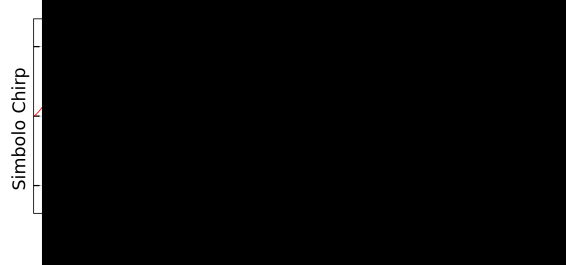
\includegraphics[width=10cm]{Time_Chirp}
        \caption{Esempio di segnale Chirp nel dominio del tempo}
\end{figure}
Per aumentare l'efficienza delle sue trasmissioni, LoRa utilizza i segnali Chirp in combinazione ad una
modulazione Spread Spectrum. Questo vuol dire che data una banda $B = [f_0,f_1]$
il segnale Chirp inviato dai dispositivi LoRa sarà distribuito in tutta la banda
$B$. Nel caso in cui il segnale,  aumentando linearmente la sua frequenza, arrivi
ad uno degli estremi della bada $f_0,f_1$  all istante $t_c$ e non potendo uscire 
dalla stessa, è costretto all'istante $t_{c+1}$ a ripartire dalla frequenza opposta a quella
dell'estremo raggiunto è possibile osservare questo fenomeno in
\hyperlink{label_in_fig_1}{$\star$}.
Utilizzando una modulazione Spread Spectrum in combinazione con i segnali di tipo
chirp, e possibile ottenere numerosi vantaggi.
\begin{figure}[h]
        \centering
                \import{Images/Eps/}{Chirp.eps_tex}
        \caption{Segnale Chirp nel dominio della frequenza}
\end{figure}
\begin{itemize}
\item Uno spettro idealmente rettangolare, il quale utilizza tutta la capacità
del canale e fornisce un ottima densità spettrale di potenza rispetto agli atri
tipi di trasmissione.
\item \textbf{Segnali di tipo Chirp} possono essere sovrapposti in modo tale da
poter variare il data-rate e l'energia per bit in modo adattativo per aumentare
l'efficienza complessiva.
\item \textbf{Hanno guadagno programmabile}, il quale permette di raggiungere
distanze considerevoli mantenendo un buon SNR .
\item  \textbf{Ottima risoluzione nel asse del tempo}, quindi ottimi per coprire
lunghe distanze.
\item \textbf{Immuni al effetto Doppler} 
\item \textbf{Immuni alle degenerazioni per effetto di multipath} \info{Trovare
termine per multipath}
\end{itemize}

Uno degli aspetti peculiari del layer fisico, è la possibilità di andare a
modificare un parametro che prende il nome di Spread Factor in modo dinamico per
massimizzare l'efficenza della comunicazione.
Lo Spread Factor è il parametro che indica quanti bit sono utilizzati in un segnale Chirp
per rappresentare un simbolo, questo vuol dire che, preso uno 
SF pari a $X$, il segnale  utilizzerà $2^X$ bit per rappresentare il simbolo a lui
associato. Variando il SF variano anche le possibili frequenze iniziali del
segnale; infatti, ogni segnale avrà $M=2^X$ frequenze iniziali possibili.
Nella documentazione tecnica fornita da Semtech troviamo 7 possibili Spread
Factor partendo dal 6SF fino ad arrivare al 12SF, ad ognuno di essi è associato un
rapporto segnale che sarà più elevato per SF maggiori \ref{tab:SNR}. 
\begin{table}[h]
        \centering
        \begin{tabular}{l|c}
                \textbf{SF}  & SNR \\
                \hline
                \emph{7}  & -7.5[dB] \\
                \emph{8}  & -10[dB]  \\
                \emph{9}   & -12.5[dB]  \\
                \emph{10} & -15[dB] \\
                \emph{11} & -17.5[dB] \\
                \emph{12} & -20[dB] \\
        \end{tabular}
        \caption{Rapporto segnale rumore dei diversi Spreading Factors}
        \label{tab:SNR}
\end{table}
\\
In combinazione allo Spreading Factor LoRa utilizza differenti lunghezze di 
banda per codificare; queste lunghezze di banda variano in base al modello di
trasmettitore utilizzato. Nel modello SX1272 tre lunghe di banda 125[KHz],
250[KHz] e 500[KHz] ed è ottimizzato per lavorare nelle frequenze che vanno
dagli  850[MHz] fino a  1[GHz]. Il modello SX1276 ha la possibilità di variare
la banda partendo da 7.8[KHz] fino a 500[KHz], offre una maggiore sensitività in
ricezione rispetto al suo predecessore ed è ottimizzato per funzionare nelle
bande degli 150[MHz] 433[MHz] e 850[MHz]-1[GHz].
Ponendoci ora nel caso in cui la banda utilizzata
nella comunicazione sia fissata a priori, una variazione dello Spread Spectrum
comporterà la necessità utilizzare il doppio del tempo per inviare il simbolo.
Nella formula \ref{eq:time_chirp} $T_s$ rappresenta il tempo necessario per
l'invio del simbolo, $X$ lo Spreading Factor usato e $B$ la banda.
Analogamente è possibile andare un incremento della banda $B$ comporterà un
incremento della velocità con cui i segnali chirp vengono trasmessi ottenendo
quindi un aumento del bit rate .
\begin{equation}\label{eq:time_chirp}
        T_s=\frac{2^{\text{X}}}{B}.
\end{equation}

\begin{figure}[h]
\centering 
\import{Images/Eps/}{Chirp_SF.eps_tex}
\caption{Comparazione simbolica dei vari SF}
\end{figure}
Un aumento del tempo impiegato per la trasmissione di un simbolo permette al
messaggio di essere più robusto alle interferenze e al rumore, è importante però
ricordare che aumentando il Spread Factor anche il numero di simboli codificabili nel
segnale  aumenterà rendendo critica la decodifica del segnale quando si è in
presenza di bassi data rate. Per questo motivo è necessario scegliere il SF in
maniera efficace, è possibile determinare in modo empirico la sensitività del
ricevitore in base al SF utilizzato secondo la formula  \improvement{Inserire Link} 
\begin{equation}
        S = -174+10\log_{10}BW + NF + SNR
\end{equation}
Dove il primo termine è dovuto al rumore termico nel ricevitore in una banda di
1[Hz] alla temperatura ambiente, $NF$ è il rumore intrinseco del ricevitore, il
quale è fissato in base all'hardware utilizzato e $SNR$ è il valore del rapporto
segnale rumore utilizzato in base alla tabella \ref{tab:SNR}

\begin{figure}[h]
        \centering 
                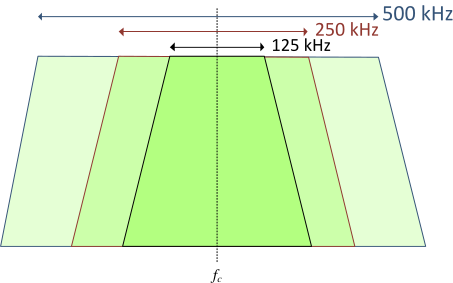
\includegraphics[width=10cm]{strong_SF}
        \caption{Lora bandwidth }
\end{figure}

Questa nuovo modo di trasmettere i vari dati porta con se molti vantaggi.
\begin{itemize}
\item La modulazione Lora è semplice da implementare nei dispositivi, quindi i
moduli radio al loro interno saranno economici.
\item Resistente alle interferenze in banda e fuori banda.
\item Resistente  all'effetto Doppler, in questo modo è possibili utilizzare
cristalli non molto accurati al interno dei devices, in modo tale da abbattere i
costi di produzione.
\item Il modulo di ricezione è altrettanto semplice da costruire, quindi non
molto costoso.
\end{itemize}
\improvement{Rivedere i vari punti e cambiare il linguaggio}
\subsection{LoRa packet}
Per ottimizzare la durata della batteria dei dispositivi, è necessario che il
devices rimanga in deep-sleep per la maggior parte del tempo. Inoltre per
utilizzare le risorse in maniera più efficace, una comunicazione LoRa è priva di
handshake e ACK. Queste scelte hanno portato all'implementazione di quello che
può essere chiamato pacchetto del layer fisico \ref{fig:phis_pack}.
Ogni pacchetto inviato è composto da:
\begin{itemize}
        \item \emph{Preambolo} data la scelta del non utilizzo di tecniche di
        handshaking e ACK, è necessario che il ricevitore sia in grado di
        sincronizzarsi con il messaggio inviato dal dispositivo. Per questo
        motivo la parte iniziale di ogni messaggio è composta da una serie di
        simboli byte utili alla sincronizzazione. La lunghezza prestabilita è di
        12 simboli.
        \item \emph{Header e CRC} l'header contiene le informazioni riguardanti
        il payload quali , la sua lunghezza , il code rate utilizzato nel
        payload e la presenza o meno del CRC. Da specifica, l'header ha sempre
        un code-rate pari a 4/8 che rappresenta la massima rindondanza con
        correlato CRC. 
        \item \emph{Payload} il quale può essere di lunghezza variabile fino ad
        un massimo di 255[byte].
        \item \emph{Payload CRC}
\end{itemize}
\begin{figure}[h]
        \centering 
                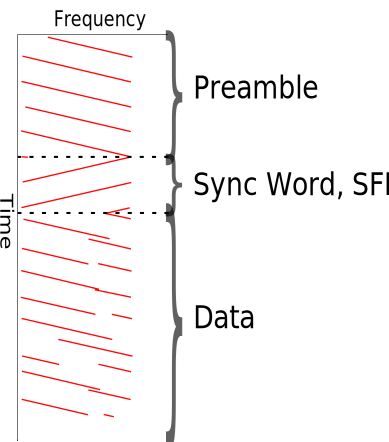
\includegraphics[width=9cm]{Chirp_Message}
        \caption{Struttura pacchetto Lora }
        \label{fig:phis_pack}
\end{figure}
In caso di specifiche stringenti, è possibile far operare i moduli LoRa in
modalità \emph{implicita}. In questa modalità, il pacchetto non utilizza
l'header; per garantire il corretto funzionamento e dunque necessario che il
payload sia di lunghezza fissata e nota al gateway al quale il messaggio è
indirizzato.
Osservando l'immagine \ref{fig:freq_lora_chirp}  è facile notare come è
strutturato un pacchetto "fisico".
La prima parte della trasmissione, nonché il preambolo  stesso è codificato con una
serie di \emph{up-chirp}. In questo modo il gateway riesce a sintonizzarsi sulla
stessa frequenza del dispositivo trasmittente.
Successivamente vengono inviati una serie di
\emph{down-chirp} i quali rappresentano l'header codificato dal layer fisico,
dove sono presenti dei bit di controloo e correzzione degli errori
L'ultima parte rappresenta il payload , in questa parte, formata solo da
\emph{UpChirp} i dati vengono codificati tramite un cambiamento istantaneo della
frequenza.
\begin{figure}[h]
        \centering 
                \includegraphics[width=9cm]{PHY_packet}
        \caption{Pacchetto codificato dal layer fisico}
        \label{fig:freq_lora_chirp}
\end{figure}
Oltre alla modulazione, LoRa specifica delle operazioni di codifica che vengono
fatte prima che il segnale venga modulato.
\begin{itemize}
        \item \textbf{Data whitening} è una tecnica utilizzata per ridurre la
        probabilità di avere lunghe sequenze di 1 e 0. Oltre a semplificare la
        decodifica, il data whitening aiuta a distribuire l'informazione in tutta la
        banda.
        \item \textbf{Forward Error Correction} è implementata tramite
        l'utilizzo dei codici di Hamming, la lunghezza della parola del codice è
        fissata e pari a 4, mentre la code-word è un parametro che può variare
        da 5 a 8.
        \item \textbf{Codice Gray} utilizzato per m \improvement{Completare}
        \item \textbf{Interliving}
\end{itemize}
La lunghezza del payload come detto prima è un numero variabile il quale dipende
da molti fattori 
\begin{equation}
        L_{payload} = 8+
        \text{max}\left(\left[\frac{8\text{PL}-4\text{SF}+44-20\text{H}}{4(\text{SF}-2\text{DE})}
        \right]+(CR+4)\, , \, 0 \right)
\end{equation}
Dove $\text{PL}$ è il numero di byte del payload iniziale, $\text{H}$ può essere
1 o 0 a seconda se il device opera in modalità "implicita" oppure no,
$\text{CR}$ è il numero di bits di parità e \text{DE} può essere 0 o 1 a seconda
dell'abilitazione o meno della funzione di \emph{low data rate}.
L'opzione di low data rate è attivabile in caso di trasmissioni lunghe e lente,
attivandola si forzerà il dispositivo trasmittente ad aumentare la stabilità
della frequenza scelta per la comunicazione .

\subsection{Chip interno}
Per quanto riguarda la struttura interna dei moduli radio, non si hanno molte
informazioni dato che la tecnologia è proprietaria di Semtech. Nella
documentazione ufficiale è presente una rappresentazione grafica dei vari
blocchi presenti al interno dei moduli radio.

\begin{figure}[h]
\centering 
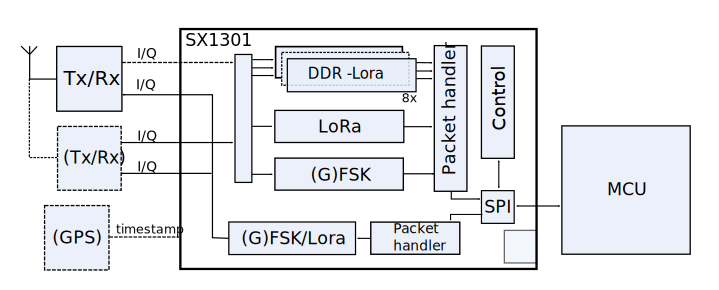
\includegraphics[width=11cm]{SX1301}
\caption{Struttura interna ricevitore SX1301}
\label{fig:sx1301}
\end{figure}

Dalla figura \ref{fig:sx1301} è evidendte che il gateway rimane in ascolto su 8 
frequenze diverse, le quali permettono di coprire tutti i vari SF. 
Tutto ciò è possibili anche grazie al fatto che i vari SF sono quasi ortogonali 
fra di loro, in questo modo il ricevitore è in grado di ricevere un pacchetto
con uno Spreading Factor $i$ anche nel caso in cui si sovrapponga ad un altro
pacchetto con Spreading Factor pari a $j$, fintanto che $i\neq j$. Questa
pseudo-ortogonalità utilizzata in LoRa, permette di utilizzare differenti SF per
ottenere un maggiore throughput rispetto a schemi di modulazione tradizionale.
Il ricevitore  SX1301 può demodulare fino ad un massimo di 8 pacchetti
contemporaneamente, questo non vuol dire che ricevitori futuri non possano
demodulare contemporaneamente un numero di pacchetti maggiore.
Oltre a ciò grazie alla modulazione utilizzata abbiamo vantaggi quali:
\begin{itemize}
\item I vari nodi della rete, possono cambiare frequenza in ogni trasmissione in
modo casuale, andando a migliorare di molto la robustezza del sistema alle varie
interferenze.
\item Non è necessario avere tabelle contenenti informazioni riguardanti il
data-rate dei vari nodi. Ogni data-rate viene demodulato contemporaneamente.
\item È possibilie utilizzare più antenne nel gateway per realizzare il
cosidetto true antenna diversity, per aumentare la robustezza al multi-path
\end{itemize}
\unsure{Riguardare ultimo punto della documentazione pagina 14}

\section{LoRaWAN}
\info[inline]{Chiedere se il termine protocollo è appropriato}
Se la scelta di utilizzare un layer fisico proprietario comporta l'utilizzo di
chip prodotti esclusivamente da Semtech, 
LoRaWAN è un protocollo MAC o \emph{media access control} utilizzabile nelle
comunicazioni che richiedono una vasta copertura di rete. Sviluppato in modo da
poter essere utilizzato per devices a basso consumo energetico, permette a
quest'ultimi la possibilità di interagire con applicazioni internet attraverso
una rete wireless a lungo raggio.
Riprendendo il modello OSI LoRaWAN può essere collocato tra il secondo e terzo
layer del sudetto modello.

\begin{figure}[h]
\centering 
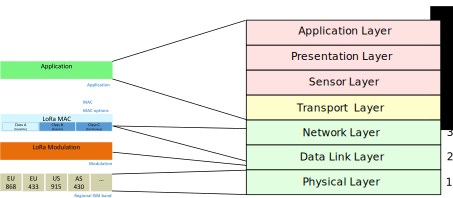
\includegraphics[width=11cm]{OSI_vs_lora}
\caption{Comparazione del modello OSI con la struttura definita in LoRaWAN}
\label{}
\end{figure}

Il protocollo LoRaWAN è sviluppato dalla LoRa Alliance e formalizzato tramite la
documentazione LoRaWAN \improvement{inserire link}
\subsection{Tipi di devices}
Nella documentazione LoRaWAN sono definite tre classi di devices possibili per
diversi tipi di utilizzo. La classe basilare è la classe \emph{A}, questo vuol
dire che in ogni dispositivo implementa questa classe. Le classi \emph{B}, e
\emph{C} sono una estensione della classe \emph{A}, questo tipo di classi sono
riservate a devices i quali hanno la possibilità di essere alimentati tramite la
rete elettrica oppure tramite fonti di energia esterne.
\begin{itemize}
        \item   \textbf{Class A} è la modalità di funzionamento predefinita. 
                In questa
                modalità il device è in grado di iniziare la comunicazione in qualsiasi istante
                di tempo. Questa classe implementa due finestre di ascolto da parte del devices
                dopo 1[s] e 2[s] dalla fine della trasmissione. Se il gateway non risponde al
                messaggio ricevuto durante uno di questi intervalli, è necessario aspettare che
                il device torni ad aprire le sue finestre di ascolto, quindi è necessario
                aspettare l'invio di un nuovo messaggio .
        \item   \textbf{Class B} sono devices che estendono le funzionalità della classe
                \emph{A}. Questi devices sono sincronizzati con la Base Station attraverso
                messaggi \emph{bacon} inviati dal gateway. Essendo sincronizzato con il gateway,
                il device è in grado di aprire finestre di ascolto nei tempo prestabilito
                potendo così essere contatto dal server.\improvement{Riscrivere}
        \item   \textbf{Class C} è anch'essa una estensione della classe \emph{A}. 
                Questa classe permette il funzionamento quasi complementare del device; infatti
                il device che opera in questa classe rimarrà continuamente in ascolto finché non
                necessità di comunicare con altri devices. Questa classe è adatta per
                comunicazioni che richiedono una bassa latenza. Ovviamente, rimanendo per la
                maggior parte del tempo in ascolto, i devices che operano con questa classe
                dovranno essere connessi ad una fonte di energia esterna 
\end{itemize}


\subsection{Frequenze}
La tecnologia LoRa opera nelle bande non licenziate dello spettro radio.  Come
accade per le più comuni tecnologie wireless WiFi, Bluetooth, ZigBee, anche LoRa
può essere utilizzata dal consumatore senza la necessità di possedere una
licenza o pagare un abbonamento.  Nonostante la diversità delle frequenze ISM
che si trovano in paese LoRaWAN supporta sia le frequenze che vanno dagli
863-868[MHz] sia la banda dei 433[MHz]. Per le frequenze centrate nella fascia
degli 860[MHz], LoRaWAN specifica tre diversi canali (868.10, 868.30 and 868.50
MHz), con una bandwidth di 125[KHz] ciascuno i quali, dovranno essere supportati
da ogni device. Inoltre ogni gateway che opera in queste frequenze dovrà
rimanere in ascolto su tutti e tre questi canali, in particolare, questi canali
formano un set comune nel quale un possibile nuovo devices che entra nella rete
comunicherà in questi canali durante la \emph{Procedura di inserimento}. Per
quanto riguarda la banda dei 433[MHz], si hanno a disposizione sempre tre tipi
diversi di canali usabili per la \emph{join procedure} i quali sono 433.175, 
433.375  433.575 MHz. Terminata la procedura, il gateway potrà dare istruzione
di utilizzare altri canali oltre ad i 3 principali.
La regolamentazione Europea impone un duty-cycle molto ristretto per l'utilizzo
delle frequenze ISM, in particolare nella banda degli 868 si è imposto
l'utilizzo di duty cycle inferiori al 1\% e per i 433 duty cycle inferiori al
0,1\%.
\begin{table}[h]
        \centering
        \begin{tabular}{l|c}
                \toprule
                Stato   & Frequenza [MHz] \\
                \hline
                Europa  & 868-870 \\
                US      & 902-928 \\
                China   & 779-787 \\
                \bottomrule
        \end{tabular}
        \caption{Bande di frequenza per le varie regioni}
\end{table}

\subsection{Sicurezza e LoRaWAN packets}
Data la necessità 
All'interno del frame \emph{PHYPayload} del pacchetto LoRa,  è il pacchetto
LoRaWAN. Questo pacchetto è strutturato nel seguente modo:
Per garantire la sicurezza nelle comunicazioni, LoRa utilizza tre diverse chiavi
di sicurezza lunghe ognuna 128[bits].
\begin{figure}[h]
\centering 
\includegraphics[width=11cm]{LoRaWAN_packet}
\caption{Stack del protocollo della rete LoRaWAN}
\label{fig:stack_lora}
\end{figure}

La topologia di rete utilizzata, è una topologia a stella, nella quale molti
dispositivi sono connessi e comunicano con uno o più base station. Le BS non
sono altro che dei ponti per poter trasmettere i messaggi ricevuto dai vari
devices all Network Server, tramite una connessione ethernet, 3G o 2G. 
Per come è strutturata la rete, un messaggio inviato
da un singolo device, può essere ricevuto e inoltrato da più BS all Network
Server.

Il NS ha il compito di interpretare e scartare i vari messaggi duplicati che
arrivano, selezionare la BS più adatta per inviare il messaggio di downlink
creando un database di tutti i vari devices presenti nella rete. Nella figura
\ref{fig:stack_lora} è rappresentato lo stack del protocollo degli end-devices,
gateway  e network-server. 

\begin{figure}[h]
\centering 
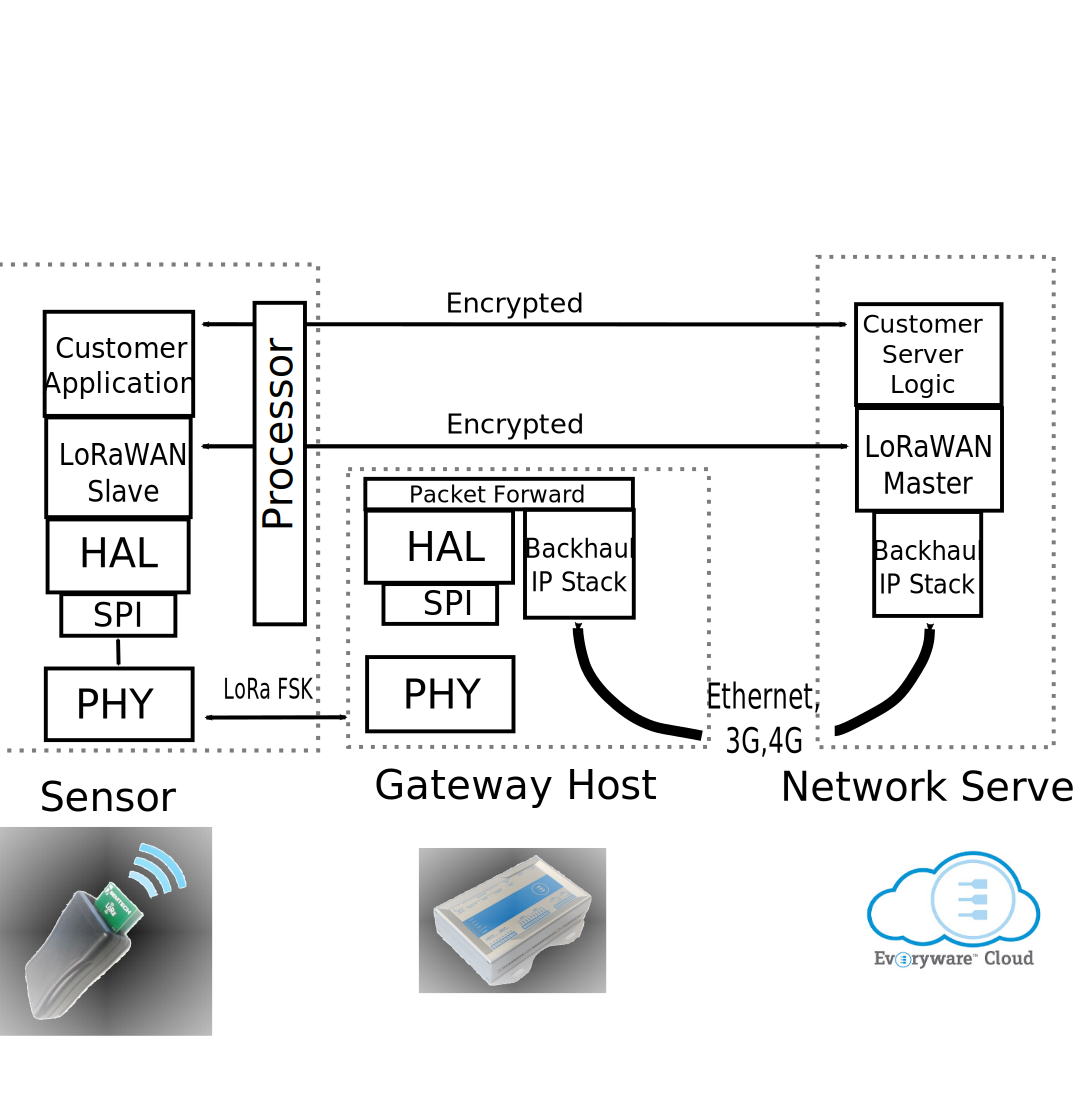
\includegraphics[width=11cm]{Lora_WAN_Stack}
\caption{Stack del protocollo della rete LoRaWAN}
\label{fig:stack_lora}
\end{figure}

\begin{figure}[h]
\centering 
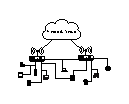
\includegraphics[width=11cm]{LPWAN_Star_network}
\caption{Struttura rete a stella LPWAN}
\end{figure}

